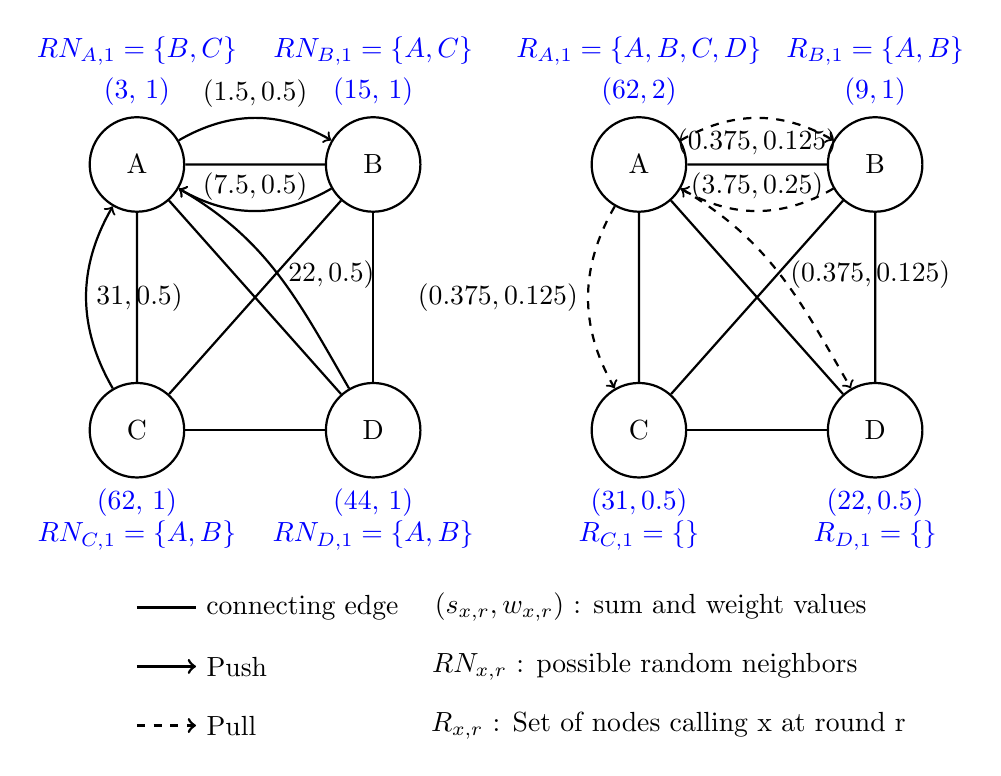
\begin{tikzpicture}[scale=0.75, thick, main node/.style={circle, draw, minimum size=1.2cm}]

    % First graph
    \node[main node] (A1) at (-1,4.5) {A};
    \node[main node] (B1) at (3,4.5) {B};
    \node[main node] (C1) at (-1,0) {C};
    \node[main node] (D1) at (3,0) {D};
    
    \node[above, color=blue] at (A1.north) {(3, 1)};
    \node[above, color=blue] at (B1.north) {(15, 1)};
    \node[below, color=blue] at (C1.south) {(62, 1)};
    \node[below, color=blue] at (D1.south) {(44, 1)};

    \node[above, color=blue] at (-1,6) {$RN_{A,1}=\{B,C\}$};
    \node[above, color=blue] at (3,6) {$RN_{B,1}=\{A,C\}$};
    \node[above, color=blue] at (-1,-2.2) {$RN_{C,1}=\{A,B\}$};
    \node[above, color=blue] at (3,-2.2) {$RN_{D,1}=\{A,B\}$};

     \node[above, color=blue] at (7.5,6) {$R_{A,1}=\{A, B, C, D\}$};
    \node[above, color=blue] at (11.5,6) {$R_{B,1}=\{A, B\}$};
    \node[above, color=blue] at (7.5,-2.2) {$R_{C,1}=\{\}$};
    \node[above, color=blue] at (11.5,-2.2) {$R_{D,1}=\{\}$};
    
    \draw (A1) -- (B1);
    \draw (A1) -- (C1);
    \draw (A1) -- (D1);
    \draw (B1) -- (C1);
    \draw (B1) -- (D1);
    \draw (C1) -- (D1);

    % Second graph
    \node[main node] (A2) at (7.5,4.5) {A};
    \node[main node] (B2) at (11.5,4.5) {B};
    \node[main node] (C2) at (7.5,0) {C};
    \node[main node] (D2) at (11.5,0) {D};
    
    \node[above, color=blue] at (A2.north) {$(62, 2)$};
    \node[above, color=blue] at (B2.north) {$(9, 1)$};
    \node[below, color=blue] at (C2.south) {$(31, 0.5)$};
    \node[below, color=blue] at (D2.south) {$(22, 0.5)$};
    
    \draw (A2) -- (B2);
    \draw (A2) -- (C2);
    \draw (A2) -- (D2);
    \draw (B2) -- (C2);
    \draw (B2) -- (D2);
    \draw (C2) -- (D2);

    \draw[->] (A1) to[out=30, in=150] node[above] {$(1.5, 0.5)$} (B1);
    \draw[->] (B1) to[out=210, in=-30] node[above] {$(7.5, 0.5)$} (A1);
    \draw[->] (C1) to[out=120, in=240] node[right] {$31, 0.5)$} (A1);
    \draw[->] (D1) to[out=120, in=-30] node[right] {$22, 0.5)$} (A1);


    
    %\draw[dashed, ->] (C1) to[out=60, in=300] node[right] {$\frac{l_{C}-l_{A}}{2}$} (A1);
    %\draw[dashed, ->] (A1) to[out=330, in=210] node[right] {$\frac{l_{C}-l_{A}}{2}$} (B1);
    

    
    \draw[dashed, ->] (A2) to[out=30, in=150] node[below] {$(0.375, 0.125)$} (B2);
     \draw[dashed, ->] (A2) to[out=240, in=120] node[left] {$(0.375, 0.125)$} (C2);
     \draw[dashed, ->] (A2) to[out=-30, in=120] node[right] {$(0.375,0.125)$} (D2);
      \draw[dashed, ->] (B2) to[out=210, in=-30] node[above] {$(3.75,0.25)$} (A2);

    % Legend in the middle below the graphs
    \begin{scope}[shift={(3,-3)}]
        % Horizontal line
        \draw (-4,0) -- (-3,0) node[right] {connecting edge};
        % Long right arrow
        \draw[->, line width=1pt] (-4,-1) -- (-3,-1) node[right] {Push};
        % Long right dashed arrow
        \draw[->, dashed, line width=1pt] (-4,-2) -- (-3,-2) node[right] {Pull};
        
        % Load notation
        \node at (4.7,0) {$(s_{x,r}, w_{x,r})$ : sum and weight values};
        \node at (4.6,-1) {$RN_{x,r}$ : possible random neighbors};
        \node at (5,-2) {$R_{x,r}$ : Set of nodes calling x at round r};
    \end{scope}

\end{tikzpicture}